\documentclass[10pt]{article}
\usepackage[margin=0.85in]{geometry}
\usepackage{graphicx}
\usepackage{booktabs}
\usepackage{amsmath}
\usepackage{xcolor}
\usepackage[hidelinks]{hyperref}
\usepackage{enumitem}
\usepackage{titlesec}
\setlist{nosep,leftmargin=*}
\titlespacing*{\section}{0pt}{7pt}{3pt}
\titlespacing*{\subsection}{0pt}{5pt}{2pt}
\setlength{\parskip}{3pt}
\setlength{\parindent}{0pt}
\setlength{\textfloatsep}{8pt}
% generated by docs/make_numbers.py -- do not edit by hand
\newcommand{\HistShpEmpty}{0.112}
\newcommand{\HistShpFull}{0.185}
\newcommand{\HistUniEmpty}{0.054}
\newcommand{\HistUniFull}{0.062}
\newcommand{\HistChainGap}{0.006}
\newcommand{\CornerShpNreset}{181}
\newcommand{\CornerUniSixHundred}{0.987}
\newcommand{\CornerShpNany}{225}
\newcommand{\CornerShpL}{225}
\newcommand{\CornerShpQ}{0.9909}
\newcommand{\CornerShpWorst}{count 6, DRAIN}
\newcommand{\QoneSpearman}{0.88}
\newcommand{\QonePearson}{0.81}
\newcommand{\QonePoints}{70}
\newcommand{\QoneVfourLastFindMax}{304}
\newcommand{\QoneVfourLastFindMin}{102}
\newcommand{\QoneVfourCrossClosedAtOneSixHundred}{3}
\newcommand{\QoneVfourCrossClosedAtTwentyFiveHundred}{1}
\newcommand{\QoneVfourCrossClosedAtThreeTwoHundred}{1}
\newcommand{\QoneVfourCrossClosedLater}{0}
\newcommand{\QoneFindsAfterClosure}{0}
\newcommand{\QoneVfourCaught}{29}
\newcommand{\QoneVoneCaught}{28}
\newcommand{\QoneVoneMissed}{write\_beats\_reset}
\newcommand{\QoneVfourCrossAtFourHundred}{80.5}
\newcommand{\QoneVfourCrossAtFifty}{44.0}
\newcommand{\QoneVfourAllAtFifty}{25.2}
\newcommand{\QoneVoneCrossMax}{72.5}
\newcommand{\QoneVoneAllAtFifty}{22.2}
\newcommand{\QoneMedianVone}{8}
\newcommand{\QoneMedianVfour}{13}
\newcommand{\QoneMedianBoundaryVone}{84}
\newcommand{\QoneMedianBoundaryVfour}{17.5}
\newcommand{\QtwoSeeds}{20}
\newcommand{\QtwoBudgetShort}{100}
\newcommand{\QtwoBudgetLong}{2,500}
\newcommand{\QtwoDirectedFind}{29}
\newcommand{\QtwoShortCrvMean}{27.80}
\newcommand{\QtwoShortCrvLow}{27.05}
\newcommand{\QtwoShortCrvHigh}{28.55}
\newcommand{\QtwoShortCrvMin}{24}
\newcommand{\QtwoShortCrvMax}{29}
\newcommand{\QtwoShortCrvSd}{1.61}
\newcommand{\QtwoShortCrvSeedOne}{28}
\newcommand{\QtwoShortCrvSeedOneHigher}{9}
\newcommand{\QtwoShortCrvSeedOneLower}{5}
\newcommand{\QtwoShortSuiteMean}{29.00}
\newcommand{\QtwoShortSuiteLow}{29.00}
\newcommand{\QtwoShortSuiteHigh}{29.00}
\newcommand{\QtwoShortSuiteMin}{29}
\newcommand{\QtwoShortSuiteMax}{29}
\newcommand{\QtwoShortSuiteSd}{0.00}
\newcommand{\QtwoShortSuiteSeedOne}{29}
\newcommand{\QtwoShortSuiteSeedOneHigher}{0}
\newcommand{\QtwoShortSuiteSeedOneLower}{0}
\newcommand{\QtwoShortCrvRelMean}{7.80}
\newcommand{\QtwoShortCrvRelLow}{7.61}
\newcommand{\QtwoShortCrvRelHigh}{7.99}
\newcommand{\QtwoShortCrvRelMin}{7}
\newcommand{\QtwoShortCrvRelMax}{8}
\newcommand{\QtwoShortCrvRelSd}{0.41}
\newcommand{\QtwoShortCrvRelSeedOne}{8}
\newcommand{\QtwoShortCrvRelSeedOneHigher}{0}
\newcommand{\QtwoShortCrvRelSeedOneLower}{4}
\newcommand{\QtwoShortCovMean}{87.93}
\newcommand{\QtwoShortCovLow}{86.88}
\newcommand{\QtwoShortCovHigh}{88.98}
\newcommand{\QtwoShortCovMin}{83.1}
\newcommand{\QtwoShortCovMax}{93.43}
\newcommand{\QtwoShortCovSd}{2.24}
\newcommand{\QtwoShortCovSeedOne}{86.39}
\newcommand{\QtwoShortCovSeedOneHigher}{13}
\newcommand{\QtwoShortCovSeedOneLower}{3}
\newcommand{\QtwoShortSeedsClosing}{0}
\newcommand{\QtwoShortSeedDependent}{6}
\newcommand{\QtwoLongCrvMean}{29.00}
\newcommand{\QtwoLongCrvLow}{29.00}
\newcommand{\QtwoLongCrvHigh}{29.00}
\newcommand{\QtwoLongCrvMin}{29}
\newcommand{\QtwoLongCrvMax}{29}
\newcommand{\QtwoLongCrvSd}{0.00}
\newcommand{\QtwoLongCrvSeedOne}{29}
\newcommand{\QtwoLongCrvSeedOneHigher}{0}
\newcommand{\QtwoLongCrvSeedOneLower}{0}
\newcommand{\QtwoLongSuiteMean}{29.00}
\newcommand{\QtwoLongSuiteLow}{29.00}
\newcommand{\QtwoLongSuiteHigh}{29.00}
\newcommand{\QtwoLongSuiteMin}{29}
\newcommand{\QtwoLongSuiteMax}{29}
\newcommand{\QtwoLongSuiteSd}{0.00}
\newcommand{\QtwoLongSuiteSeedOne}{29}
\newcommand{\QtwoLongSuiteSeedOneHigher}{0}
\newcommand{\QtwoLongSuiteSeedOneLower}{0}
\newcommand{\QtwoLongCrvRelMean}{8.00}
\newcommand{\QtwoLongCrvRelLow}{8.00}
\newcommand{\QtwoLongCrvRelHigh}{8.00}
\newcommand{\QtwoLongCrvRelMin}{8}
\newcommand{\QtwoLongCrvRelMax}{8}
\newcommand{\QtwoLongCrvRelSd}{0.00}
\newcommand{\QtwoLongCrvRelSeedOne}{8}
\newcommand{\QtwoLongCrvRelSeedOneHigher}{0}
\newcommand{\QtwoLongCrvRelSeedOneLower}{0}
\newcommand{\QtwoLongCovMean}{99.84}
\newcommand{\QtwoLongCovLow}{99.71}
\newcommand{\QtwoLongCovHigh}{99.96}
\newcommand{\QtwoLongCovMin}{99.06}
\newcommand{\QtwoLongCovMax}{100}
\newcommand{\QtwoLongCovSd}{0.28}
\newcommand{\QtwoLongCovSeedOne}{100}
\newcommand{\QtwoLongCovSeedOneHigher}{0}
\newcommand{\QtwoLongCovSeedOneLower}{6}
\newcommand{\QtwoLongSeedsClosing}{14}
\newcommand{\QtwoLongSeedDependent}{0}
\newcommand{\QtwoCrvAgreeFrom}{400}
\newcommand{\QtwoSuiteAgreeFrom}{50}
\newcommand{\CrossAagree}{64}
\newcommand{\CrossAtotal}{64}
\newcommand{\CrossBagree}{32}
\newcommand{\CrossBtotal}{32}

\newcommand{\code}[1]{\texttt{#1}}
\begin{document}
\sloppy

\begin{center}
{\Large\bfseries Project 1: Constrained-Random Verification of a Synchronous FIFO}\\[3pt]
EEE 4701 / EEE 5703 \;$\cdot$\; Team: Brandon Zabawa and Leo \;$\cdot$\; packet rev 8b9d934 \;$\cdot$\; November 2026
\end{center}

\noindent\fbox{\parbox{\dimexpr\linewidth-2\fboxsep}{\small\textbf{AI disclosure.} AI was used to help finish this task.}}

\section{Summary}
We verified the course FIFO (\code{dut/fifo.sv}, FWFT, \code{WIDTH}$=$\code{DEPTH}$=8$) against \code{dut/specs/fifo.md} with a layered cocotb environment, pyvsc constrained-random stimulus, and a cocotb-coverage model of 10 coverpoints, 3 crosses, 2 justified ignore bins and 4 illegal checks. The graduate extension answers two questions from the graduate-study menu: Q1 (Brandon) and Q2 (Leo).

\begin{center}\small
\begin{tabular}{lp{11.9cm}}
\toprule
Released pool (\code{craft\_mutate}) & \textbf{8/8} \\
Our own 24-mutant pool & \textbf{21/24} (2 survivors are outside the spec's defined behavior, 1 is equivalent) \\
Functional coverage & \textbf{100\%} (213/213 bins) on the sign-off seed at cycle 975; 100\% merged over seeds 1--10; 9/10 seeds alone \\
Reproducibility & identical stimulus digests and coverage on all 30 regression runs before and after this revision's rewrite \\
Q1: coverage vs.\ bugs & coverage and finds correlate (Spearman $\rho=\QoneSpearman$) only through short budgets: every findable bug falls by cycle \QoneVfourLastFindMax{}, while the cross keeps closing for thousands of cycles \\
Q2: seed spread & at \QtwoBudgetShort{} cycles the CRV test finds \QtwoShortCrvMin--\QtwoShortCrvMax{} of 32 across \QtwoSeeds{} seeds (mean \QtwoShortCrvMean, 95\% CI [\QtwoShortCrvLow, \QtwoShortCrvHigh]); at \QtwoBudgetLong{} every seed finds \QtwoLongCrvMax; the whole suite finds \QtwoShortSuiteMax{} on every seed \\
\bottomrule
\end{tabular}
\end{center}

\section{Verification plan and traceability}
\code{vplan.md} numbers the spec into requirements R1--R9 (reset; write iff \code{wr\_en \&\& !full}; read iff \code{rd\_en \&\& !empty}; simultaneous r+w; flags; FIFO order; port ranges; the corner list; parameters) and maps them to 14 features F1--F14, each with a priority and a verification method. Every test names the features it covers (T1 directed smoke, T2 security reset race, T3 constrained-random sign-off) and every feature has at least one test. The plan states its closure targets before any measurement (100\% of the model, at least 90\% on the hidden pool, every survivor classified) and lists six ambiguities with their resolutions. Two drive results below: \code{rd\_data} while empty is undefined (risk 2), and rule 3's ``continuously shows the current head'' is read literally (risk 3).

\section{Environment}
\textbf{Layering (\code{tb/}).} The \emph{driver} drives on the falling edge and owns the clock; it never checks. The \emph{monitor} reads every pin back, inputs included, into a \code{PinSnapshot}, so a driver bug cannot hide behind a matching expectation. The \emph{scoreboard} is a reference queue (\code{FifoModel}, a deque). Each cycle it steps the model with the monitor's view of the inputs on the pre-edge state, then asserts \code{count}, \code{full}, \code{empty}, and the head whenever the model is non-empty. Coverage is sampled from the scoreboard's own \code{CycleRecord}, so what is covered is what was checked. The layers come from our HW4 suite; the only change in kind is a \textbf{second sample point}: 1\,ns after the new inputs are driven and before the edge, the outputs must still equal the model's current state. That check found a mutant no stimulus could expose at the post-edge sample (Section~\ref{sec:mut}).

\textbf{Reuse and readability.} The same \code{FifoEnv} serves the directed tests, the CRV test, the regression runner, the graduate-study runner, and other parameter sets (\code{DEPTH=5 WIDTH=4} closes 100\% on seed~1; \code{DEPTH=16 WIDTH=16} runs green). In this revision every layer was rewritten to read top-down in plain words (\code{drive\_one\_cycle}, \code{check\_before\_edge}, \code{OPERATION\_MIX}); Section~\ref{sec:revision} shows the rewrite changed no behavior.

\section{Constrained-random stimulus}
\textbf{Legality.} Every \code{(wr\_en, rd\_en)} pair is legal at every occupancy (a write while full is dropped, a read while empty ignored) and reset is a legal input. So no constraint is needed for legality and none can break it. The constraints only shape.

\textbf{Transaction (\code{crv/transactions.py}).} \code{wr\_en}, \code{rd\_en}, \code{wr\_data} are random. \code{count} (the occupancy the DUT reports) and \code{phase} (FILL/DRAIN) are non-random and set before each \code{randomize()}. One uniform draw \code{roll}$\in$0..19 is mapped to an operation by hard implications inside \code{if\_then / else\_if / else\_then} on \code{count} and \code{phase}:

\begin{center}\small
\begin{tabular}{llcccc l}
\toprule
region & phase & write-only & both & read-only & idle & intent\\
\midrule
count$\le$1 & FILL & 60\% & 25\% & 10\% & 5\% & push writes away from empty\\
count$\le$1 & DRAIN & 10\% & 20\% & 55\% & 15\% & park at empty: read-while-empty\\
2..6 & FILL / DRAIN & 40 / 10\% & 45\% & 10 / 40\% & 5\% & simultaneous r+w, drift to target\\
count$\ge$7 & DRAIN & 10\% & 25\% & 60\% & 5\% & push reads away from full\\
count$\ge$7 & FILL & 55\% & 20\% & 10\% & 15\% & park at full: write-while-full\\
\bottomrule
\end{tabular}
\end{center}

The phase flips with probability 0.05 per cycle spent at the target boundary (mean dwell 20 cycles). \code{wr\_data} is 40\% data corners (0x00, 0xFF, 0x55, 0xAA). The sign-off profile v4 adds resets at 1/30 per cycle at empty or full and 1/120 elsewhere, with the enables on a reset cycle drawn from two unconstrained pyvsc bits.

\textbf{Induced distribution.} Before trusting it we measured it. Three pyvsc behaviors forced the design above (Section~\ref{sec:ctm}): a \code{dist} inside \code{if\_then} is applied unconditionally, a bounded field is not uniform, and a guarded reset field fired at 10--16$\times$ its intended rate. The induced operation rates now match the table to within 0.03. Fig.~\ref{fig:hist} shows the occupancy they induce; it agrees with an exact Markov-chain model of the table to within \HistChainGap{} at every occupancy.

\begin{figure}[h]
\centering
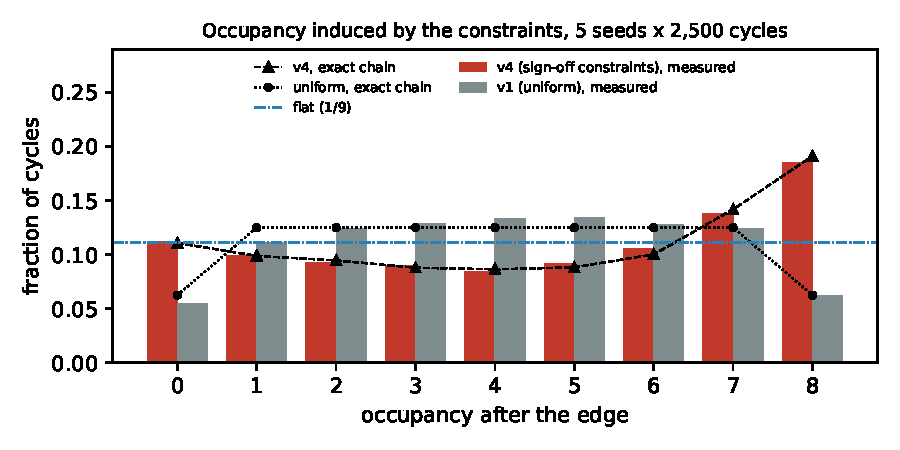
\includegraphics[width=0.66\linewidth]{../extension/figures/occupancy_hist.pdf}
\vspace{-5pt}
\caption{Occupancy induced by v4 against uniform (v1), measured over 5 seeds $\times$ 2,500 cycles, with the exact-chain prediction.}
\label{fig:hist}
\end{figure}

\section{Coverage model and closure}
\textbf{Model (\code{coverage\_model/model.py}).} Coverpoints: post-edge occupancy (9 bins), operation (4), pre-edge occupancy class (empty/one/mid/almost\_full/full), outcome (8, separating requested from performed, so dropped and ignored operations are bins), accepted-write data class (5), pointer wrap (2), occupancy class on wrap edges (5), reset occupancy (3), enables during reset (4), and a (slot, bit, value) march over every popped word (128). Crosses: X1 occupancy class $\times$ operation (20 bins, \emph{no} ignore bins: \code{(full, write)} and \code{(empty, read)} are spec-defined corners); X2 wrap $\times$ occupancy class (8 bins; \code{(rd\_wrap, full)} and \code{(wr\_wrap, empty)} are ignored because rules 2--4 make them unreachable); X3 reset occupancy $\times$ enables (12 bins, the security thread). Illegal checks: a count change other than rules 2--4 allow, \code{full}$\wedge$\code{empty}, both pointers wrapping on one edge, occupancy outside 0..8.

\noindent\begin{minipage}{\linewidth}
\textbf{Convergence argument (\code{closure.md}).}
\begin{center}\small
\begin{tabular}{lp{5.6cm}rrp{4.2cm}}
\toprule
profile & change & per-seed & merged & holes left (5 seeds, 2,500 cycles)\\
\midrule
v1 & uniform transaction, no resets & 92.49\% & 92.49\% & 11/12 reset-cross bins\\
v2 & boundary-shaped transaction, resets 1/400 & 93.9--98.1\% & 99.06\% & \code{rst\_x\_en (empty, wr/both)}\\
v3 & reset rate raised at the boundaries & 98.1--99.1\% & 100\% & 0/5 seeds close alone\\
v4 & partial-occupancy resets restored, uniform enables during reset & 99.5--100\% & 100\% & 4/5 close alone\\
\bottomrule
\end{tabular}
\end{center}
\end{minipage}
On the sign-off seed the model reaches 86.4\% at 100 cycles and 97.2\% at 400. It closes at cycle 975, and the last bin is the reset cross \code{(partial, wr)}. v3 is the instructive step: raising resets at the boundaries closed \code{(full,*)} but starved partial occupancy and opened three new holes. Every hole was closed by changing a constraint or the reset policy, never by a directed test aimed at a bin. Over seeds 1--10, nine close alone at 2,500 cycles; seed~4 misses \code{(partial, both)} and closes at 4,000 cycles, so the gap is budget, not reachability.

\section{Mutation quality and survivors}\label{sec:mut}
The released pool is found 8/8. To see past it we wrote 24 hidden-style bugs in the harness format: 6 overlapping-enable traps, 4 reset faults, 2 pointer faults, 6 boundary or flag faults, 3 storage-cell faults, 2 behaviors outside the spec's defined window, and 1 logically equivalent rewrite. The suite finds 21. The HW4 directed suite and our first CRV cut both found 20.

\begin{center}\small
\begin{tabular}{p{3.9cm}p{2.5cm}p{9.5cm}}
\toprule
survivor & gap & why it survived, and what would catch it\\
\midrule
\code{empty\_bypass\_\allowbreak leaks\_input} & observability (spec) & \code{rd\_data} shows the input bus while empty. The spec defines the head only when \code{!empty}, so nothing may check it. Catch: a spec decision, then a stability check on \code{rd\_data} while empty, or an information-flow check that \code{rd\_data} does not depend on same-cycle \code{wr\_data}.\\
\code{empty\_reads\_zero} & observability (spec) & Same window. Under this spec it is a legal implementation; a check that flagged it would over-read the spec.\\
\code{full\_from\_pointers} & equivalent & \code{(wr\_ptr==rd\_ptr)\&\&(cnt!=0)} $\equiv$ \code{cnt==DEPTH}. No simulation can tell them apart; an \code{sby} invariant proof would classify it formally.\\
\code{write\_beats\_reset} (v1 only) & reachability & v1 never asserts \code{wr\_en} during reset. Found by T2 and by v4, whose reset-cross bins name exactly this state.\\
\code{head\_shows\_input\_\allowbreak on\_simul\_at\_one} (HW4 and first cut) & observability (sampling point) & At the post-edge sample its \code{rd\_data} equals the true head; it differs only between edges. Found by the second sample point, which rule 3 (``continuously'') justifies.\\
\bottomrule
\end{tabular}
\end{center}

\section{Security and trust thread}
The spec defines reset but not a write or read asserted on the same edge. T2 drives exactly that, with data inside and both pointers away from slot 0, and then a read and a write racing at the empty boundary. It asserts that reset wins, that the count is 0, and that no pre-reset data, and not the marker written during reset, ever reaches the head. Cross X3 makes ``a write asserted during reset at each occupancy class'' a coverage obligation; closing it is what makes CRV find \code{write\_beats\_reset}. The two empty-window survivors are the security residue: a design that leaked data onto \code{rd\_data} while empty would pass, and only a spec change can close that.

\section{Graduate extension: the distribution the constraints induce}
\textbf{Distribution against uniform.} Pooled over 5 seeds (Fig.~\ref{fig:hist}), v4 puts \HistShpEmpty{} of cycles at empty and \HistShpFull{} at full. Uniform puts \HistUniEmpty{} and \HistUniFull{}, which is \emph{half} its interior mass: at the boundaries a uniform ``both'' request becomes a one-sided move away from that boundary. Uniform random is therefore biased \emph{against} the states where the FIFO's gating logic lives.

\textbf{A constraint that reaches a named corner.} Corner: \code{full} with a simultaneous read and write requested. With an absorbing state added to the exact chain, P(hit within $N$ draws) is a matrix power whose entries are the constraint table. From reset, v4 exceeds $p=0.99$ at $N=\CornerShpNreset$ draws (uniform: \CornerUniSixHundred{} at 600). Splitting the run into windows of $L$ draws and taking the worst starting state's hit chance $q_L$ gives
\[ P(\text{hit within } N) \;\ge\; 1-(1-q_L)^{\lfloor N/L\rfloor} \]
from \emph{any} state; the chain yields $q_{\CornerShpL}=\CornerShpQ$ (worst start \CornerShpWorst), so $P>0.99$ within $N=\CornerShpNany$ draws from any state.

\section{Q1: Does closing coverage track finding bugs? \normalfont\small(Brandon Zabawa)}\label{sec:q1}
\textbf{Claim (could be wrong).} On this FIFO, cross-coverage closure tracks found/total only up to a small budget. Past it, finds stand still while the cross keeps closing, so a closed cross certifies stimulus breadth, not detection. The claim is refuted if found/total keeps rising with the cross right up to closure.

\textbf{Setup.} Profiles v1 (uniform) and v4 (sign-off), seeds 1--5, 7 doubling budgets from 50 to 3,200 CRV cycles, released pool (8) plus our own pool (24). \code{extension/detection\_runner.py} runs the CRV test once per (profile, seed, mutant) in study mode (no drain, no gates) and records the cycle of the first failing check; a run with budget $B$ is an exact prefix of the 3,200-cycle run, so a mutant is found at $B$ iff it first fails at a cycle $\le B$. The course harness agrees with this shortcut on \CrossAagree/\CrossAtotal{} verdicts (Section~\ref{sec:revision}). \code{extension/q1\_coverage\_vs\_bugs.py} makes Fig.~\ref{fig:q1} and every number below.

\begin{figure}[h]
\centering
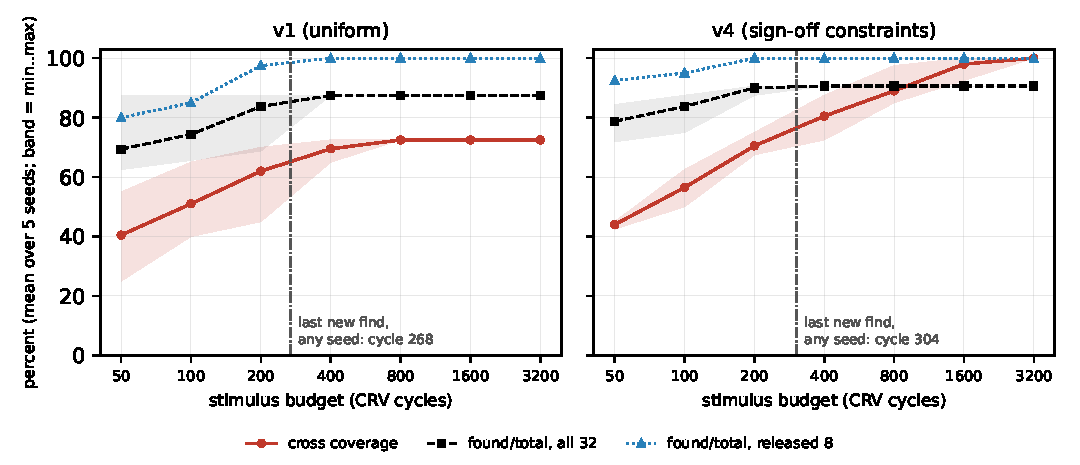
\includegraphics[width=0.86\linewidth]{../extension/figures/q1_curves.pdf}
\vspace{-5pt}
\caption{Q1: cross coverage and found/total on one budget axis (mean over 5 seeds; bands are min..max).}
\label{fig:q1}
\end{figure}

\textbf{Results.} Over all \QonePoints{} (profile, seed, budget) points, cross coverage and found/total correlate (Pearson $r=\QonePearson$, Spearman $\rho=\QoneSpearman$), but the correlation comes from the short budgets. Under v4, every findable mutant falls by cycle \QoneVfourLastFindMax{} on every seed (the last new find lands between cycle \QoneVfourLastFindMin{} and \QoneVfourLastFindMax{}); at 400 cycles the cross is only at \QoneVfourCrossAtFourHundred\% on average, and it first reaches 100\% at 1,600 cycles on \QoneVfourCrossClosedAtOneSixHundred{} seeds, at 2,500 on \QoneVfourCrossClosedAtTwentyFiveHundred{} and at 3,200 on \QoneVfourCrossClosedAtThreeTwoHundred. Mutants first found after the cross closed: \QoneFindsAfterClosure. Under v1 both curves stall: the cross never passes \QoneVoneCrossMax\%, v1 catches \QoneVoneCaught{} of 32, and the one reachable mutant it misses (\code{\QoneVoneMissed}) sits behind the one cross it never closes (\code{rst\_x\_en} stays at 1 of 12 bins: v1 issues no resets after the opening one). Shaping moves \emph{boundary} bugs earlier, not every bug: the median first-failure cycle of our boundary-class mutants is \QoneMedianBoundaryVone{} under v1 and \QoneMedianBoundaryVfour{} under v4, while over all found mutants the medians are close (\QoneMedianVone{} and \QoneMedianVfour), because most mutants fail within the first few cycles under either profile.

\textbf{What it means for sign-off.} A reviewer should now believe that an \emph{open} cross was informative: the missed bug sat behind it. A reviewer should still not believe that \emph{closing} the cross added detection; past a few hundred cycles it bought breadth only. Report coverage and found/total side by side. \textbf{Limits:} one small design (every boundary is reached within a few hundred cycles), one pool written by the suite's authors, doubling budgets locate the knee only to within a factor of two.

\section{Q2: How much does the seed matter? \normalfont\small(Leo)}\label{sec:q2}
\textbf{Claim (could be wrong).} The seed matters only at short budgets. At \QtwoBudgetShort{} CRV cycles found/total spreads across seeds; at the \QtwoBudgetLong-cycle sign-off budget every seed scores the same, so our reported seed-1 score is not a lucky seed. Refuted if the long-budget distribution still has spread, or if seed~1 sits above the 95\% interval.

\textbf{Setup.} Profile v4, seeds 1--\QtwoSeeds, budgets \QtwoBudgetShort{} and \QtwoBudgetLong{} cycles, both pools (32 mutants), from the same runner as Q1 (seeds 1--5 are shared). Two views: \emph{CRV only} (the part the seed controls) and \emph{whole suite} (T1+T2, which use no randomness and are run once per mutant, plus the CRV test), which is what the harness grades. The interval is a 95\% $t$-interval for the mean, $\bar x \pm t_{0.975,\,n-1}\, s/\sqrt{n}$. \code{extension/q2\_seed\_spread.py} makes Fig.~\ref{fig:q2} and Table~\ref{tab:q2}.

\begin{figure}[h]
\centering
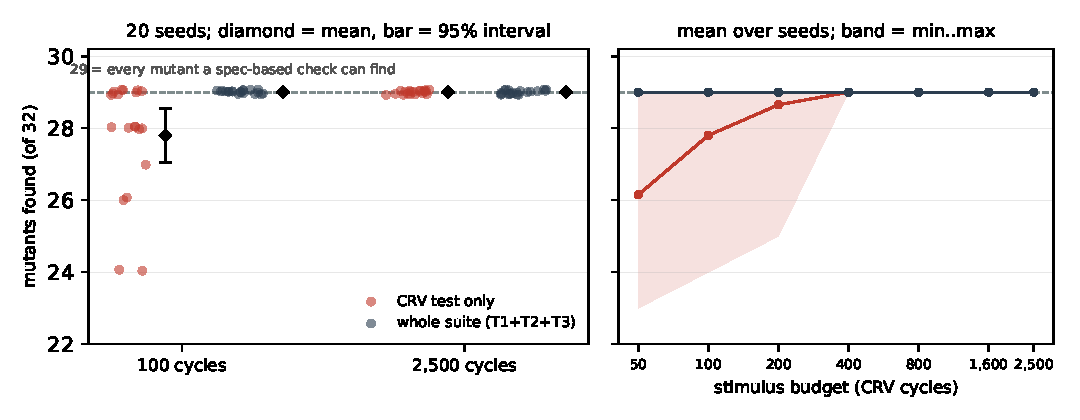
\includegraphics[width=0.86\linewidth]{../extension/figures/q2_seed_spread.pdf}
\vspace{-5pt}
\caption{Q2: found/total per seed at the two budgets (left; diamond = mean, bar = 95\% interval) and across every checkpoint (right).}
\label{fig:q2}
\end{figure}

\begin{table}[h]\centering\small
\begin{tabular}{rlcccc}
\toprule
budget & view (of 32) & mean & 95\% interval & min--max & seed 1\\
\midrule
\QtwoBudgetShort & CRV only & \QtwoShortCrvMean & [\QtwoShortCrvLow, \QtwoShortCrvHigh] & \QtwoShortCrvMin--\QtwoShortCrvMax & \QtwoShortCrvSeedOne\\
\QtwoBudgetShort & whole suite & \QtwoShortSuiteMean & [\QtwoShortSuiteLow, \QtwoShortSuiteHigh] & \QtwoShortSuiteMin--\QtwoShortSuiteMax & \QtwoShortSuiteSeedOne\\
\QtwoBudgetLong & CRV only & \QtwoLongCrvMean & [\QtwoLongCrvLow, \QtwoLongCrvHigh] & \QtwoLongCrvMin--\QtwoLongCrvMax & \QtwoLongCrvSeedOne\\
\QtwoBudgetLong & whole suite & \QtwoLongSuiteMean & [\QtwoLongSuiteLow, \QtwoLongSuiteHigh] & \QtwoLongSuiteMin--\QtwoLongSuiteMax & \QtwoLongSuiteSeedOne\\
\bottomrule
\end{tabular}
\caption{Q2: found/total over \QtwoSeeds{} seeds. Released pool alone, CRV only: \QtwoShortCrvRelMean{} of 8 at \QtwoBudgetShort{} cycles, \QtwoLongCrvRelMean{} at \QtwoBudgetLong.}
\label{tab:q2}
\end{table}

\textbf{Results.} At \QtwoBudgetShort{} cycles the seed decides \QtwoShortSeedDependent{} of the 32 verdicts: the CRV score ranges \QtwoShortCrvMin--\QtwoShortCrvMax{} (s.d.\ \QtwoShortCrvSd), and seed~1 scores \QtwoShortCrvSeedOne{} (\QtwoShortCrvSeedOneHigher{} seeds score higher, \QtwoShortCrvSeedOneLower{} lower). From \QtwoCrvAgreeFrom{} cycles on, every seed agrees; at \QtwoBudgetLong{} the distribution is a single value, \QtwoLongCrvMax/32, so the interval collapses to it. The seed still moves \emph{coverage} at \QtwoBudgetLong{} (\QtwoLongSeedsClosing{} of \QtwoSeeds{} seeds close 100\% before the final drain, minimum \QtwoLongCovMin\%), not finds. The whole suite scores \QtwoShortSuiteMax/32 on every seed at both budgets, because the directed tests alone find \QtwoDirectedFind{} of 32, every mutant any check against this spec can find.

\textbf{What it means for sign-off.} Our reported score is not a lucky seed: at the graded budget every one of \QtwoSeeds{} seeds gives the same found/total, and the 3 misses are the survivors of Section~\ref{sec:mut}. A reviewer should not read this as ``the seed never matters'': it matters for coverage closure at 2,500 cycles and for detection at short budgets, and a larger design with a slower knee would carry that spread to longer runs. \textbf{Limits:} a $t$-interval assumes roughly normal data, which a bounded count with few distinct values is not; the min--max range is the honest statement at \QtwoBudgetShort{} cycles. One design, one pool, \QtwoSeeds{} seeds.

\section{What this revision fixed, tested, and ran}\label{sec:revision}
\begin{itemize}
\item \textbf{Readability rewrite, no behavior change.} Every file in \code{tb/}, \code{crv/}, \code{coverage\_model/} and \code{test\_fifo\_p1.py} was rewritten with full-word names. All 30 regression runs (sign-off seeds 1--10; convergence v1--v4 $\times$ seeds 1--5) reproduce the earlier stimulus digests, coverage and occupancy exactly, and the harness again scores 8/8 and 21/24. The histogram and corner-bound numbers also reproduce exactly.
\item \textbf{A bug in our own study instrumentation.} \code{reset\_keeps\_count} leaves \code{empty} at X, so reading it raises \code{ValueError}, not an assertion. The earlier study labeled this mutant \code{build/crash}; our first rewrite recorded it as a survivor. The study mode now records any exception as the failure, so it reads ``found at cycle 0''.
\item \textbf{A reproducibility gap closed.} The earlier extension numbers (correlation, median detection cycles) were read from a \code{summary.json} that no script in the repo produced. Every extension number now regenerates from \code{extension/}, and \code{docs/make\_numbers.py} writes every number in this report.
\item \textbf{The method checked against the course harness.} Check A: the harness in study mode at budgets 100 and 800 agrees with the prefix method on \CrossAagree/\CrossAtotal{} verdicts. Check B: the harness in its graded configuration agrees with ``directed OR CRV within 2,500'' on \CrossBagree/\CrossBtotal.
\item \textbf{Upload failure.} Uploading the folder sent all of \code{.git/} and every raw log, and each file came back \code{502 Bad Gateway}. A \code{.gitignore} now keeps regenerable output out of the repo, and the submission zip leaves out \code{.git/}.
\end{itemize}

\section{Check the Machine}\label{sec:ctm}
We had the assistant draft the constraint block and the coverage model, and wrote a prediction before each run (\code{ai\_log.md}). (1)~Branch-local \code{vsc.dist} under \code{if\_then}: predicted unguarded; measured P(\code{wr\_en})$=$0.64/0.66/0.63 in three regions written as 0.90/0.80/0.20. \emph{Confirmed}; fixed with hard implications on one uniform draw. (2)~\code{rangelist} roll: predicted uniform; measured end deciles at 18\%/16\%. \emph{Refuted}; fixed with an unguarded equal-weight \code{dist}. (3)~A guarded reset field: predicted too frequent; measured 16\% where 1.6\% was intended. \emph{Confirmed}; moved to the sequence layer. (4)~Coverage-model draft: we predicted it would ignore the drop and ignore corners (refuted) and that it would mis-build the march (confirmed: one name defined twice). (5)~The ported scoreboard: we predicted CRV alone would beat the directed suite on our pool. It tied at 20/24, which led to the second sample point. (6)~This revision's rewrite: we predicted renaming pyvsc constraint blocks could reorder the solver and change the stimulus. \emph{Refuted}: 30/30 digests identical. We also did not predict that the rewrite's narrower exception handler would turn one found mutant into a false survivor; the per-mutant comparison against the old data caught it.

\section{Reproducibility and limits}
Every run logs its seed and a SHA-1 digest of the stimulus; \code{SEED=$n$ make SIM=icarus} replays it. \code{crv/regress.py} regenerates every coverage table, the scripts in \code{extension/} every graduate number, and \code{README.md} lists each command. \textbf{Not verified:} \code{rd\_data} while empty; parameter sets other than 8/8 beyond a smoke run; behavior between our two sample points; misreadings the reference model shares with the RTL; Verilator was not rerun in this revision (the earlier run was green under Verilator 5.020).

\end{document}
